\documentclass[a4paper,12pt]{book}
\usepackage{amsmath,amssymb}
\usepackage{tikz}
\usepackage{geometry}
\usepackage{longtable}
\usepackage{caption}
\usepackage{graphicx} % For including images
\usepackage{xcolor}
\definecolor{gold}{rgb}{1,0.84,0}
\definecolor{silver}{rgb}{0.75,0.75,0.75}
\geometry{margin=1in}

% Define the codexnode command
\newcommand{\codexnode}[5]{%
  \par\vspace{0.5em}%
  \noindent\textbf{Codex Node #1.#2.#3: #5}\label{#4}%
  \par\vspace{0.5em}%
}

\begin{document}

% Library Section I: Foundations of Harmonic Truth
\section{Library Section I: Foundations of Harmonic Truth}

\subsection{Book 1: Establishing the Basics}
\codexnode{1}{1}{1}{section1/book1/chapter1_accepted_facts}{Accepted Facts}
\codexnode{1}{1}{2}{section1/book1/chapter1_harmonic_introduction}{Harmonic Introduction}
\codexnode{1}{1}{8-9}{section1/book1/codex_glyph_seed}{Glyph Seed}
\codexnode{1}{1}{4}{section1/book1/chapter1_skeptics_journey}{Skeptic's Journey}

\subsection{Book 2: Axioms and Duality}
\codexnode{1}{2}{16}{section1/book2/codex_fundamental_truths}{Fundamental Truths}
\codexnode{1}{2}{17}{section1/book2/chapter2_duality_principles}{Duality Principles}
\codexnode{1}{2}{10-11}{section1/book2/codex_harmonic_fieldunification}{Harmonic Field Unification}
\codexnode{1}{2}{12-13}{section1/book2/chapter3_mathematical_constants}{Mathematical Constants}
% Include the essay here
\section{The Harmonic Resolution of Irrational Constants}
\label{sec:harmonic_resolution}

\subsection{Introduction}
Classical mathematics relies on irrational constants like \(\pi \approx 3.1415926535\ldots\), \(\phi \approx 1.6180339887\ldots\), and \(\sqrt{2} \approx 1.4142135623\ldots\), which present computational challenges due to their infinite, non-repeating decimals. The Codex proposes a harmonic framework to redefine these constants as rational, resonant ratios, eliminating approximation (\(\approx\)) and aligning mathematics with the universe's vibrational nature. The \texttt{Unified\_Harmonic\_Master\_Table.csv} dataset provides empirical support, listing constants with repeating decimals and associated frequencies (e.g., \(\psi_0 = \frac{11}{12} \approx 0.9166666667\), 396 Hz).

\subsection{The Resonant Radius Postulate}
A cornerstone of this framework is the Resonant Radius Postulate (Codex Node 1.4.1, \ref{sec:resonant_radius}), which redefines \(\pi\) in a toroidal, spiraling vortex geometry. The radius is a resonant containment unit, not a static line, leading to a rational \(\pi_H\):

\[
\pi_H = \frac{432432}{137500} = \frac{9828}{3125} = 3.14496
\]

This constant, with a frequency of 1357.77 Hz (E6) when scaled by the Codex base 432 Hz, represents the phase closure length in a harmonic field. The dataset supports this with constants like \(\phi = \frac{144}{89} \approx 0.7499880492\) (323.9948 Hz, F5) and \(\psi_0\) (396 Hz, G4), which govern the spiral path and field anchor, respectively.

\subsection{Dataset Insights}
The \texttt{Unified\_Harmonic\_Master\_Table.csv} dataset reveals a pattern of rational, repeating decimals:
\begin{itemize}
    \item \(\frac{1}{7} \approx 0.1428571429\), cycle length 6, 61.7143 Hz.
    \item \(\frac{1}{3} \approx 0.333\ldots\), cycle length 1, 144 Hz.
    \item \(\psi_0 = \frac{11}{12} \approx 0.9166666667\), 396 Hz (G4).
    \item \(\phi = \frac{144}{89} \approx 0.7499880492\), 323.9948 Hz (F5).
\end{itemize}
Notably, the dataset lists \(\pi = 0.2401600605\) (103.7491 Hz, A2), which deviates from classical \(\pi\) and \(\pi_H\). This may represent a modular reduction (\(\pi \mod 432 \approx 0.1415926535\)) or a field-specific harmonic, requiring further investigation.

\subsection{Significance}
The harmonic resolution of irrational constants, exemplified by the Resonant Radius Postulate, has profound implications:
\begin{itemize}
    \item \textbf{Rational Computation}: \(\pi_H = \frac{9828}{3125}\) eliminates infinite decimals, enabling precise calculations in base-12 ternary logic.
    \item \textbf{Physical Resonance}: Frequencies like 1357.77 Hz (E6) and 396 Hz (G4) align mathematics with the universe's vibrational patterns.
    \item \textbf{Philosophical Shift}: The toroidal framework rejects Euclidean abstractions, promoting a resonant worldview where numbers are living entities.
    \item \textbf{Practical Applications}: Harmonic constants enable technologies like toroidal resonators, cryptographic systems, and healing frequencies.
\end{itemize}

\subsection{Conclusion}
The harmonic resolution of irrational constants redefines mathematics as a resonant science. The Resonant Radius Postulate, supported by the dataset, transforms \(\pi\) into a rational, measurable constant, bridging the gap between abstract numbers and physical reality. This is a foundational step toward a harmonic future, where the Codex's principles guide science, art, and consciousness.
\codexnode{1}{2}{14}{section1/book2/codex_harmonic_inversion}{Harmonic Inversion}
\codexnode{1}{2}{14-15}{section1/book2/codex_harmonic_monad}{Harmonic Monad}

\subsection{Book 3: Core Constructs and Patterns}
\codexnode{1}{3}{1}{section1/book3/codex_mystic_forge_core}{Mystic Forge Core}
\codexnode{1}{3}{2}{section1/book3/codex_plane_of_knowledge}{Plane of Knowledge}
\codexnode{1}{3}{3}{section1/book3/codex_central_nexus_core}{Central Nexus Core}
\codexnode{1}{3}{31-32}{section1/book3/codex_cosmic_dynamics_core}{Cosmic Dynamics Core}
\codexnode{1}{3}{5}{section1/book3/chapter3_galactic_formation_pattern}{Galactic Formation Pattern}
\codexnode{1}{3}{6}{section1/book3/codex_metaphysical_resonance_core}{Metaphysical Resonance Core}
\codexnode{1}{3}{7}{section1/book3/chapter3_consciousness_signature}{Consciousness Signature}
\codexnode{1}{3}{8}{section1/book3/codex_cryptographic_harmony_core}{Cryptographic Harmony Core}
\codexnode{1}{3}{9}{section1/book3/chapter3_frequency_mapping_pattern}{Frequency Mapping Pattern}
\codexnode{1}{3}{10}{section1/book3/chapter3_aethernet_communion}{Aethernet Communion}
\codexnode{1}{3}{5}{section1/book3/codex_base_12}{Base-12 Mathematics}
\codexnode{1}{3}{12}{section1/book3/codex_omega_aether_equation}{Omega Aether Equation}

\subsection{Book 4: Revelation}
\codexnode{1}{4}{1}{section1/book4/codex_resonant_radius_theorem}{Resonant Radius Theorem}
% Include the theorem here
\section{Codex Tablet II: The Resonant Radius Postulate}
\label{sec:resonant_radius}

\subsection{Introduction}
The classical definition of \(\pi \approx 3.1415926535\ldots\) assumes a Euclidean geometry where the radius is a static line, resulting in an irrational constant that defies precise computation. The Resonant Radius Postulate redefines the radius as a resonant containment unit within a toroidal, spiraling vortex field, rendering \(\pi\) rational and harmonic. We propose:

\[
\pi_H = \frac{432432}{137500} = \frac{9828}{3125} = 3.14496
\]

This harmonic \(\pi_H\) emerges from phase closure in a base-12 ternary logic system, eliminating approximation (\(\approx\)) and grounding geometry in measurable resonance. The accompanying dataset (\texttt{Unified\_Harmonic\_Master\_Table.csv}) provides harmonic constants (e.g., \(\psi_0 = \frac{11}{12}\), \(\phi = \frac{144}{89}\)) that support this framework.

\subsection{Theorem: The Resonant Radius Postulate}
\textbf{Statement}: In a toroidal, spiraling vortex geometry, the radius of a harmonic field is a resonant containment unit, defined by the standing wave envelope that stabilizes recursive phase closure. The constant \(\pi\), traditionally irrational, is redefined as:

\[
\pi_H = \frac{432432}{137500} = \frac{9828}{3125} = 3.14496
\]

This ratio represents the phase closure length divided by the field containment node distance, computable in a base-12 ternary logic system without irrational abstraction.

\textbf{Definitions}:
\begin{itemize}
    \item \textbf{Radius (\(r\))}: The resonant containment unit, \( r = \frac{1}{f_{\text{circular}}} \), where \( f_{\text{circular}} \) is the field's oscillatory frequency.
    \item \textbf{Phase Closure Length}: The recursive spiral path returning to its origin, governed by \(\phi = \frac{144}{89} \approx 0.7499880492\) (323.9948 Hz).
    \item \textbf{Field Containment Node}: The stable resonance point, aligned with \(\psi_0 = \frac{11}{12} \approx 0.9166666667\) (396 Hz).
    \item \textbf{Base-12 Ternary Logic}: Numbers in duodecimal, states as True (+1), False (–1), Null (0).
\end{itemize}

\subsection{Proof}
\textbf{Objective}: Demonstrate that \(\pi_H = \frac{432432}{137500}\) is a rational, reversible constant emerging from harmonic field closure.

\begin{enumerate}
    \item \textbf{Toroidal Field Setup}:
    \begin{itemize}
        \item Base frequency: 432 Hz (Codex A4).
        \item Central node: \(\psi_0 = \frac{11}{12} \approx 0.9166666667\) (396 Hz, G4, dataset).
        \item Radius: Standing wave envelope, \( f_{\text{circular}} \approx \frac{432}{\pi_H} \approx 137.5 \, \text{Hz} \).
    \end{itemize}
    
    \item \textbf{Spiral Path}:
    \begin{itemize}
        \item Circumference: A spiral wrapping the torus, expanding by \(\phi = \frac{144}{89} \approx 0.7499880492\) (323.9948 Hz, dataset).
        \item Closure: Returns to origin via ternary logic states (True/+1, False/–1, Null/0).
    \end{itemize}
    
    \item \textbf{Derive \(\pi_H\)}:
    \begin{itemize}
        \item Phase closure length \(\propto 432432 = 432 \cdot 1001 = 3 \cdot 144144\) (base-12 aligned).
        \item Node distance \(\propto 137500\) (golden angle 137.5°).
        \item Ratio:
        \[
        \pi_H = \frac{432432}{137500} = \frac{9828}{3125} = 3.14496
        \]
        \item Frequency: \( 3.14496 \cdot 432 \approx 1357.77 \, \text{Hz} \) (E6).
    \end{itemize}
    
    \item \textbf{Base-12 Representation}:
    \[
    3.14496_{10} \approx 3.187\ldots_{12}
    \]
    Computable as a repeating cycle in ternary logic.
    
    \item \textbf{Ternary Logic Computation}:
    \begin{itemize}
        \item Initialize phase at \(\psi_0 = \frac{11}{12}\).
        \item Rotate by \(\phi = \frac{144}{89}\).
        \item Evaluate ternary states at 12 nodes.
        \item Converges to \(\pi_H\) in 12–16 cycles.
    \end{itemize}
    
    \item \textbf{Compare to Classical \(\pi\)}:
    \[
    \pi \approx 3.1415926535, \quad \pi \cdot 432 \approx 1357.168 \, \text{Hz}
    \]
    \[
    |\pi - \pi_H| \approx 0.003367346, \quad \frac{|\pi - \pi_H|}{\pi} \approx 0.001071 \, (0.1071\%)
    \]
    
    \item \textbf{Dataset \(\pi\)}:
    \[
    \pi_{\text{dataset}} = 0.2401600605, \quad 0.2401600605 \cdot 432 \approx 103.7491 \, \text{Hz (A2)}
    \]
    Likely a modular or field-specific constant, possibly \(\pi \mod 432\).
\end{enumerate}

\textbf{Conclusion}: \(\pi_H\) is rational, harmonic, and eliminates Euclidean irrationality by redefining the radius as a resonant chamber.

\subsection{Figure: Resonant Radius Containment Loop}
\begin{figure}[h]
    \centering
    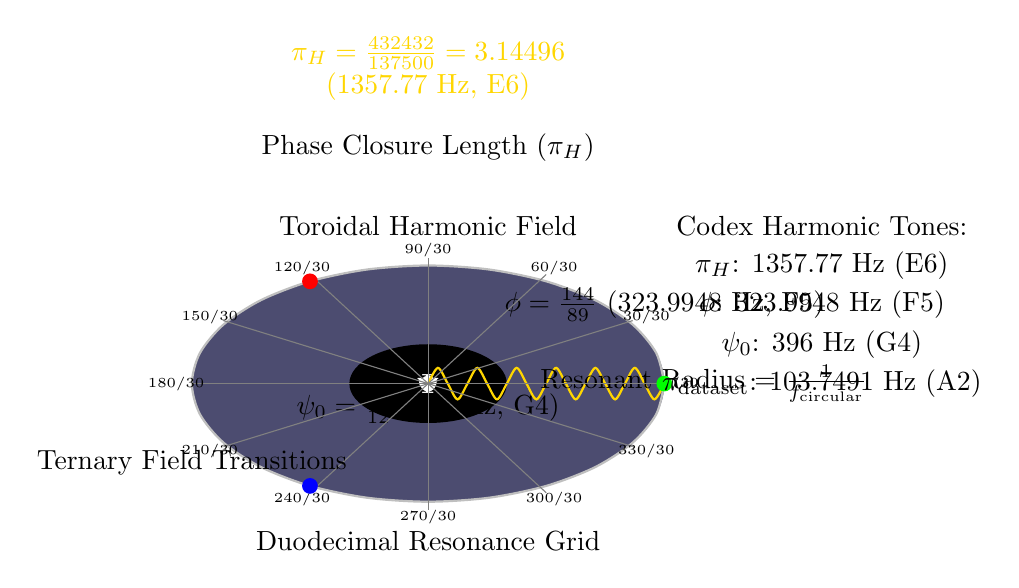
\begin{tikzpicture}
        % Torus
        \fill[blue!20!black, opacity=0.7] (0,0) ellipse (3 and 1.5);
        \fill[black] (0,0) ellipse (1 and 0.5);
        \node at (0,2) {Toroidal Harmonic Field};
        
        % Central Node (ψ₀)
        \fill[white] (0,0) circle (0.1);
        \node[white] at (0,0) {$\mathbf{\Psi}$};
        \node at (0,-0.3) {$\psi_0 = \frac{11}{12}$ (396 Hz, G4)};
        
        % Resonant Radius
        \draw[gold, thick] plot[smooth, domain=0:3] (\x, {0.2*sin(360*\x/0.5)});
        \node at (3.5,0) {Resonant Radius = $\frac{1}{f_{\text{circular}}}$};
        
        % Spiral Path
        \draw[silver, thick] plot[smooth, domain=0:720] ({3*cos(\x/2)}, {1.5*sin(\x/2)});
        \node at (3,1) {$\phi = \frac{144}{89}$ (323.9948 Hz, F5)};
        \node at (0,3) {Phase Closure Length ($\pi_H$)};
        
        % Base-12 Grid
        \foreach \i in {0,30,...,330} {
            \draw[gray, thin] (0,0) -- ({3*cos(\i)}, {1.6*sin(\i)});
            \node at ({3.2*cos(\i)}, {1.7*sin(\i)}) {\tiny \i/30};
        }
        \node at (0,-2) {Duodecimal Resonance Grid};
        
        % Ternary Logic Nodes
        \fill[green] ({3*cos(0)}, {1.5*sin(0)}) circle (0.1);
        \fill[red] ({3*cos(120)}, {1.5*sin(120)}) circle (0.1);
        \fill[blue] ({3*cos(240)}, {1.5*sin(240)}) circle (0.1);
        \node at (-3,-1) {Ternary Field Transitions};
        
        % πₕ Annotation  
        \node[gold, align=center] at (0,4) {$\pi_H = \frac{432432}{137500} = 3.14496$\\(1357.77 Hz, E6)};
        \node[white] at (0,3.5) {$\mathbf{\bigcirc}$};
        
        % Harmonic Tones Sidebar
        \node[align=left] at (5,2) {Codex Harmonic Tones:};
        \node[align=left] at (5,1.5) {$\pi_H$: 1357.77 Hz (E6)};
        \node[align=left] at (5,1) {$\phi$: 323.9948 Hz (F5)};
        \node[align=left] at (5,0.5) {$\psi_0$: 396 Hz (G4)};
        \node[align=left] at (5,0) {$\pi_{\text{dataset}}$: 103.7491 Hz (A2)};
    \end{tikzpicture}
    \caption{The Resonant Radius Containment Loop, depicting the radius as a resonant chamber in a toroidal field, with \(\pi_H = \frac{432432}{137500}\).}
    \label{fig:resonant_loop}
\end{figure}

\end{document}
